% !TEX encoding = UTF-8 Unicode
% !TEX root = thesis.tex

\chapter{Data and Methodology}
\label{ch:method}

This chapter describes how the data are produced, how the monitoring and
modelling layers are constructed, and which methods, metrics, and tools are used
to address the four research questions (RQ1--RQ4) set out in the Introduction. It also
explains and justifies the main design choices. The central methodological
decision is a \emph{simulation-first} strategy: the primary data are generated
using a custom 3GPP-compliant 5G NR Standalone handover simulator, while publicly
available drive-test measurements are used mainly to calibrate and sanity-check
the simulator; they are not the primary training source. The reason for this
choice is practical. Publicly available 5G Standalone datasets generally do not
expose handover control parameters (such as time-to-trigger, hysteresis, or A3
offset) together with the resulting mobility outcomes. A controlled simulation
environment therefore provides a more suitable way to generate labelled
configuration--performance data and to study drift and anomaly behaviour under
known conditions.

\section{Research design and scope}
\label{sec:design}

The study is organised as a pipeline of controlled experiments. A simulator
generates multi-phase timelines in which drift and anomalies are introduced at
predefined times, allowing the resulting behaviour to be analysed under
controlled conditions. Four analysis layers are then built on top of this data:
(i) unsupervised anomaly detection on handover KPI windows, (ii) concept-drift
detection on KPI streams, (iii) a drift-aware adaptive monitor that updates the
anomaly detector when a drift detector fires (subject to a cooldown), and (iv) a
configuration--performance surrogate that links handover parameters to mobility
outcomes and supports the analysis of possible reconfiguration strategies. Real
measurements are used at two points only: to calibrate the simulator's
radio-layer behaviour, and as an external face-validity check.
Figure~\ref{fig:framework} gives a high-level overview of how these layers fit
together.

\begin{figure}[p]
\centering
\IfFileExists{img/framework_overview.svg}{%
  \includesvg[inkscapelatex=false,width=\linewidth,height=0.92\textheight,keepaspectratio]{framework_overview}%
}{%
  \fbox{\parbox[c][5cm][c]{0.82\linewidth}{\centering\ttfamily framework\_overview\\[4pt]%
  \normalfont\small Placeholder: export \texttt{thesis/docs/framework\_overview.puml}
  to \texttt{img/framework\_overview.svg}.}}%
}
\caption[Overview of the drift-aware handover monitoring framework]{Overview of
the proposed anomaly- and drift-aware handover monitoring framework: a
simulation-first data layer, a monitoring layer that runs anomaly and
concept-drift detection in parallel, a drift-triggered adaptation layer based on
self-supervised filtered retraining, and a configuration--performance and
decision layer that recommends a reconfiguration with calibrated uncertainty
(own elaboration).}
\label{fig:framework}
\end{figure}

The scope follows two binding decisions. First, the entire pipeline is restricted
to \emph{5G NR Standalone intra-RAT inter-gNB Xn handover}. Each cell in the
19-cell layout is modelled as a distinct gNB, such that all handovers
correspond to inter-gNB Xn handovers (TS~38.300~\S9.2.3.2,
TS~38.331~\S5.5.4)~\cite{ts38300,ts38331}. NSA, intra-gNB, N2-based, and
inter-RAT handovers remain outside the scope of this thesis. Second, the
monitored KPI family is restricted to \emph{mobility KPIs}: the handover success
rate (HOSR), standardized as an NG-RAN KPI in TS~28.554~\S6.6~\cite{ts28554},
together with the handover failure rate, radio-link-failure (RLF) rate and
ping-pong rate, which have no TS~28.554 KPI definition and are instead computed
from the simulator's event log following the mobility-robustness conventions of
TR~36.839 and TS~28.313~\cite{tr36839,ts28313}, plus
the underlying radio measurements (serving and neighbour RSRP/RSRQ/SINR).
Service-quality KPIs such as throughput and latency are excluded because the
simulator implements the L1/L3 control plane but does not include a full L2 MAC
scheduling layer. As a result, scheduler-dependent QoS behaviour cannot be
represented in a sufficiently realistic or standard-compliant manner. Although
scheduler-related effects may indirectly influence mobility performance under
congestion conditions, the objective of this thesis is to study mobility-related
anomalies and concept drift primarily at the RRC/RRM level. The analysis
therefore focuses on mobility KPIs and radio measurements that are directly
associated with handover behaviour.

\section{Data sources}
\label{sec:data}

Two data sources drive the methodology (Table~\ref{tab:datasets}). The simulator
is the primary source of training and evaluation data. NordicDat, a public
operator drive-test set, is the calibration target for the radio layer and also
provides a real-telemetry segment for the external face-validity check.

\begin{table}[ht]
\centering
\caption{Data sources and their roles (own elaboration).}
\label{tab:datasets}
\begin{tabular}{@{}lll@{}}
\toprule
Source & Role & Nature \\
\midrule
Simulator  & Primary training/evaluation data & Synthetic 5G NR SA (3GPP-compliant) \\
NordicDat  & Radio-layer calibration + face validity & Real drive-test (5G-NSA / LTE) \\
\bottomrule
\end{tabular}
\end{table}

A third public set, the Bangladesh LTE drive-test logs, is \emph{not} a
methodological data source: it does not enter calibration or any model and is
used only in an exploratory data report to confirm that the simulator's
handover-event rates are of the same order of magnitude as a real network. Being
LTE rather than NR~SA, it is out of calibration scope and is mentioned here only
for completeness.

Real and simulated samples are never merged. Calibration is a one-way comparison
of marginal distributions, and every simulated row is tagged \texttt{ran\_type =
NR\_SA} so that the two populations remain separable. NordicDat's
\texttt{op1/5G-NSA/LTE\_B20} segment ($\approx$43k samples) is the closest
publicly available 5G-flavoured radio reference and is the calibration target;
its LTE segments are retained only as cross-RAN sanity references.

\section{The 5G NR handover simulator}
\label{sec:simulator}

A custom micro-simulator was built in MATLAB rather than adopting a full-stack
network simulator such as ns-3 5G-LENA or Simu5G. The handover scope here is
narrow (A3 event, RLF, ping-pong) and does not need PDCP/RLC/MAC fidelity, so a
focused implementation that maps closely onto the relevant 3GPP clauses keeps the
model transparent and testable: each mechanism corresponds to a specific clause
and is covered by a unit test. The simulator runs in three stages per user equipment
(UE): it places the cells and generates a trajectory, it turns that geometry into
per-tick radio measurements, and it runs the handover state machine on those
measurements. The three stages are described in turn below, and
Figure~\ref{fig:simulator-flow} summarises the overall data flow from the
configuration inputs to the parquet outputs and ground-truth labels.

\begin{figure}[ht]
\centering
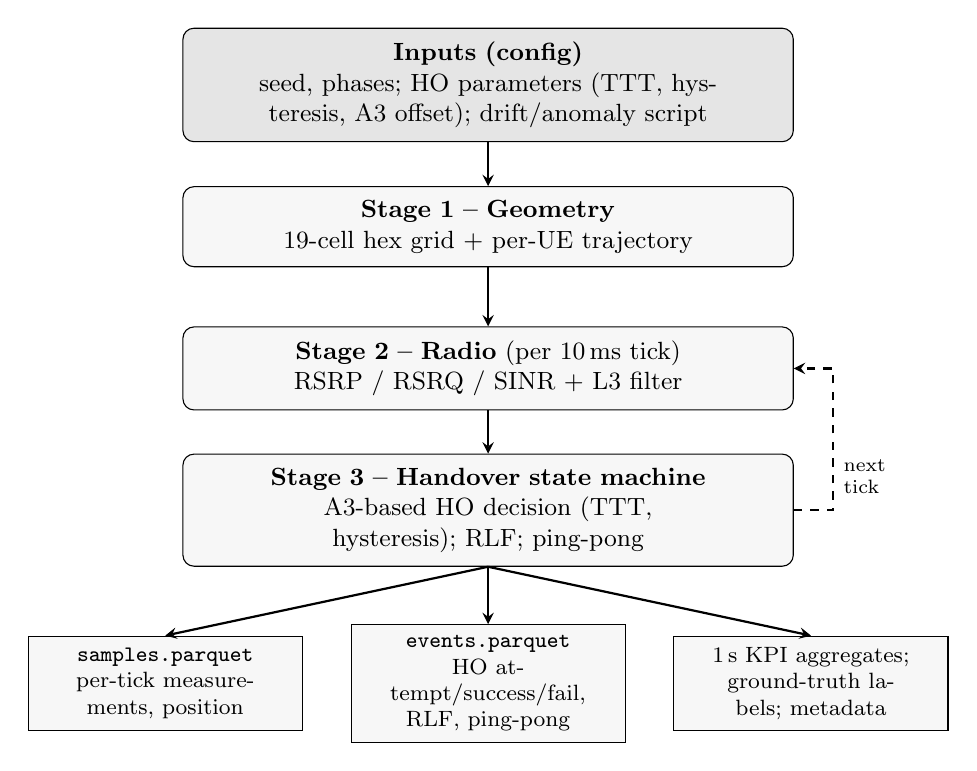
\begin{tikzpicture}[
  font=\small,
  box/.style={rectangle, rounded corners, draw, align=center, text width=7.4cm,
              inner sep=5pt, minimum height=9mm, fill=black!3},
  io/.style={rectangle, rounded corners, draw, align=center, text width=7.4cm,
             inner sep=5pt, minimum height=9mm, fill=black!10},
  ofile/.style={rectangle, draw, align=center, text width=3.2cm, font=\footnotesize,
                inner sep=4pt, minimum height=12mm, fill=black!3},
  arr/.style={->, >=stealth, thick}
]
% configuration input and the three-stage pipeline (central column)
\node[io]  (in) at (0,0)    {\textbf{Inputs (config)}\\ seed, phases; HO parameters (TTT, hysteresis, A3 offset); drift/anomaly script};
\node[box] (s1) at (0,-1.8) {\textbf{Stage 1 -- Geometry}\\ 19-cell hex grid $+$ per-UE trajectory};
\node[box] (s2) at (0,-3.6) {\textbf{Stage 2 -- Radio} (per 10\,ms tick)\\ RSRP / RSRQ / SINR $+$ L3 filter};
\node[box] (s3) at (0,-5.4) {\textbf{Stage 3 -- Handover state machine}\\ A3-based HO decision (TTT, hysteresis); RLF; ping-pong};
% outputs, split into the separate artefacts the run writes
\node[ofile] (o1) at (-4.1,-7.6) {\texttt{samples.parquet}\\ per-tick measurements, position};
\node[ofile] (o2) at ( 0.0,-7.6) {\texttt{events.parquet}\\ HO attempt/success/fail, RLF, ping-pong};
\node[ofile] (o3) at ( 4.1,-7.6) {1\,s KPI aggregates;\\ ground-truth labels; metadata};
\draw[arr] (in) -- (s1);
\draw[arr] (s1) -- (s2);
\draw[arr] (s2) -- (s3);
\draw[arr] (s3.south) -- (o1.north);
\draw[arr] (s3.south) -- (o2.north);
\draw[arr] (s3.south) -- (o3.north);
\draw[arr, dashed] (s3.east) -- ++(0.5,0) |- (s2.east)
      node[pos=0.12, right, font=\scriptsize, align=left]{next\\ tick};
\end{tikzpicture}
\caption[Data flow of the 5G NR SA handover simulator]{Data flow of the 5G NR SA
handover simulator. Configuration and a scenario script (drift and anomaly
injection) drive three stages: \emph{geometry} (19-cell hexagonal grid, each
cell a separate gNB, with a per-UE Random-Direction trajectory); per-tick
\emph{radio} modelling (RSRP/RSRQ/SINR from the TR~38.901 channel model with
LoS/NLoS, path loss and spatially correlated shadowing, smoothed by the layer-3
filter); and the \emph{handover state machine} (Event~A3 with time-to-trigger,
the T310/N310/N311 radio-link-failure timers, and ping-pong detection). The loop
is evaluated per 10\,ms tick and writes three parquet artefacts together with
ground-truth labels and metadata for the analysis pipeline (own elaboration).}
\label{fig:simulator-flow}
\end{figure}

\paragraph{Topology and deployment.}
The scenario is a 19-cell two-tier hexagonal grid (a centre cell plus two
surrounding rings of six and twelve), with an inter-site distance of 500\,m and
an omnidirectional antenna at each cell centre. The layout and inter-site distance follow the 3GPP Urban
Macro reference scenario~\cite{tr38913}; the radio settings use common
urban-macro evaluation assumptions: carrier 3.5\,GHz (band n78), 100\,MHz
bandwidth carried on 273 resource blocks at 30\,kHz subcarrier
spacing~\cite{ts38104}, base-station height 25\,m and UE height 1.5\,m (the
TR~38.901 UMa defaults~\cite{tr38901}), transmit power 49\,dBm, antenna gain
8\,dBi and a UE noise figure of 7\,dB. Each
of the 19 cells is treated as a separate gNB, so every handover the simulator
produces is, by construction, an inter-gNB Xn handover.

\paragraph{Trajectory.}
Each UE moves in a straight line at a constant speed: it starts at a random point
inside the deployment area, picks a random direction, and walks for the duration
of the phase, so its displacement is exactly speed times duration. This keeps the
ground truth simple and reproducible (everything is fixed by the seed). When a
long timeline carries a UE from one phase into the next, only its end position is
kept and a fresh direction is drawn for the new phase (the Random-Direction
model). Re-drawing the direction matters in practice: keeping the same heading
made UEs walk in a straight line off the cell footprint after a few phases and
collapse the received power, so the direction is reset at every phase boundary,
and any UE that would leave the area is simply respawned at a random point.

\paragraph{Radio measurements.}
For every tick and every cell, the simulator computes RSRP, RSRQ and SINR from
the 3GPP TR~38.901 channel model~\cite{tr38901}.
First, a line-of-sight (LoS) or non-line-of-sight (NLoS) state is drawn per cell
from the TR~38.901 LoS-probability formula and is correlated over distance so it
does not flicker tick to tick. Second, the path loss is the TR~38.901 Urban Macro
formula (Table~7.4.1-1), which is a two-slope function of distance with a
breakpoint and a separate, higher NLoS branch. Third, shadow fading is added as a
spatially correlated random field: rather than drawing an independent value per
sample, the simulator builds a smooth two-dimensional field (decorrelation
distance 37\,m, standard deviation 4\,dB in LoS and 6\,dB in NLoS) so that nearby
positions see similar fading, as real shadowing does. From these, RSRP is the
transmit EIRP minus path loss minus shadowing (normalised to a single resource
element), the wideband RSSI is the sum of all cell powers plus thermal noise, and
RSRQ and SINR follow their standard definitions (RSRQ $= N\cdot$RSRP$/$RSSI; SINR
$=$ serving-cell power over the sum of the other cells plus noise), consistent
with TS~38.215~\cite{ts38215}. The Urban Micro street-canyon model is implemented
as the alternative used by the channel-swap drift scenario (D-2). Fast
(symbol-level) fading is not modelled, because it averages out over the
measurement window and does not affect handover-event timing.

\paragraph{Handover state machine.}
The control plane is evaluated once per 10\,ms tick and follows the NR procedure
clause by clause. The raw per-cell measurements are first smoothed by the
layer-3 filter of TS~38.331~\S5.5.3.2, an exponential moving average
$F_n = (1-\alpha)F_{n-1} + \alpha M_n$ with the standard
$\alpha = 1/2^{k/4}$ ($k=4$, i.e.\ $\alpha = 0.5$). On the filtered values the
simulator evaluates Event~A3 of TS~38.331~\S5.5.4.4, whose entry condition is
that a neighbour exceeds the serving cell by the hysteresis plus the A3 offset
($M_n - \mathrm{Hys} > M_s + \mathrm{Off}$; the per-cell offset terms are set to
zero in this work). A neighbour that satisfies the condition accumulates time;
once it has held for the time-to-trigger, a handover to that neighbour fires (at
most one per tick), the UE spends a short execution interval detached, and on
completion the target becomes the serving cell. In parallel, radio-link failure
is tracked by the T310 state machine of TS~38.331~\S5.3.10: when the serving SINR
stays below an out-of-sync threshold ($-8$\,dB) for $N310=6$ ticks the T310 timer
(1\,s) starts, recovery needs $N311=2$ in-sync ticks above $-6$\,dB, and if T310
expires an RLF is declared and the UE re-establishes on the strongest cell.
Finally, a handover that returns the UE to the cell it just left within a short
window is logged as a ping-pong, in line with the mobility-robustness conventions
of TR~36.839~\cite{ts38331,tr36839}. The baseline configuration is TTT~256\,ms,
hysteresis 2\,dB and A3 offset 0\,dB. One simplification is worth stating: the
10\,ms tick is finer than the spec's $\approx$200\,ms layer-1 measurement period,
so the filter and the failure counters react somewhat faster than in a real UE;
the logic is faithful, the time constants are not.

\paragraph{Outputs.}
Each run writes two parquet streams plus a metadata file. \texttt{samples.parquet}
holds the per-UE, per-tick radio measurements and position;
\texttt{events.parquet} is the per-event log of handover attempt, success and
failure, RLF and ping-pong, each row carrying the active control parameters and
pre/post signal snapshots. A one-second per-cell aggregate (RSRP/SINR
percentiles, event counts, HOSR) is also produced for the drift streams. A single
schema with canonical \texttt{snake\_case} names is shared by the simulator and
the Python pipeline, so the same column means the same thing everywhere.

\section{Calibration against real measurements}
\label{sec:calibration}

Calibration is intended to show that the simulator's radio layer produces
distributions broadly \emph{compatible} with real 5G measurements; this is
sufficient when the simulator is used as independent training data, and no
stronger claim of statistical identity is made. The serving-cell RSRP, RSRQ
and SINR marginals are compared against the NordicDat \texttt{op1/5G-NSA/LTE\_B20}
segment with the two-sample Kolmogorov--Smirnov statistic
(\texttt{scipy.stats.ks\_2samp}), the two-sample form of the classical KS
goodness-of-fit statistic~\cite{massey1951ks}. The KS statistic, together
with a 200-replicate bootstrap 95\% confidence interval and the median offset
$\Delta p_{50}$ (sim median minus real median), is the reported quantity.
P-values are deliberately not used as the headline metric: at tens of thousands
of samples per side any non-zero KS statistic gives a vanishing p-value, so it
carries no information at this scale.

A $3\times3$ grid over inter-site distance and trajectory area indicated that the
default TR~38.901 configuration, chosen before inspecting the real data, already
provides the closest fit among the grid points. RSRP and SINR match closely
(KS~0.175 and 0.192, median offsets $+3.1$\,dB and $-2.2$\,dB). RSRQ retains a
residual mismatch (KS~0.467)
that is insensitive to channel parameters; it is load-driven rather than
channel-driven, since the v0 model uses a deterministic interference assumption,
and it is documented as a known limitation. The handover control plane itself is
\emph{not} calibrated against real handover logs, because no public 5G~SA
handover-event dataset exists; instead it is verified against the specification
through the simulator's unit tests.

\section{Scenario design: drift and anomaly injection}
\label{sec:scenarios}

A key advantage of the simulator is that drift and anomalies can be introduced at
controlled times with ground-truth labels, which is difficult to obtain from real
data. A \emph{timeline} is a concatenation of phases: a clean baseline warm-up so the
detectors can learn ``normal'', a sequence of drift and anomaly phases separated
by baseline-recovery gaps, and a steady-state tail for post-drift evaluation.

\paragraph{Drift scenarios.}
Four intra-NR drift types are scripted, each starting from baseline and applying
one transformation at a phase boundary: D-1 traffic-load shift (UE-density
change), D-2 channel-model swap (UMa~$\rightarrow$~UMi, i.e.\ cell
densification), D-3 mobility shift (mean UE speed change, e.g.\ $10\rightarrow25$\,m/s),
and D-4 reconfiguration (the operator pushes new TTT/hysteresis/A3-offset
values). D-4 changes only the control plane and therefore provides the most
direct signal for the configuration--performance surrogate. All four are
intra-5G-NR and stay within the scope defined in Section~\ref{sec:design}.

\paragraph{Anomaly scenarios.}
Four anomaly types are injected. These are the ground-truth events that the five
detectors of Section~\ref{sec:anomaly-method} are later asked to recover (the
count of four refers to the injected fault types, not to the number of
detectors). Each type corrupts the per-UE measurement stream before the handover
loop runs, so that the injection produces genuine downstream effects rather than
only a flag in a table. A-1 (RLF burst) lowers the SINR on all cells for the
affected UEs by enough to push the serving cell below the failure threshold; A-2
(measurement glitch) freezes the UE's RSRP at a constant value, mimicking a stuck
sensor; A-3 (interference spike) subtracts SINR from specific cells, so every UE
that sees those cells is affected; and A-5 (slow degradation) adds a slow linear
SINR decline on a single UE. Each injection is labelled with its time window and
the UEs and/or cells it affects, and this label is the ground truth for the
detection benchmark.

\paragraph{Timelines and labelling.}
Production timelines are generated deterministically by a parametric generator
(\texttt{tools/gen\_timeline.py}) given a seed and the desired number of phases,
drifts and anomalies; anomalies are forbidden in the head-baseline phases so the
detectors always get a clean training window. The main timeline used for the
benchmarks, \texttt{timeline\_medium}, has 30 phases of 60\,s (1\,800\,s total),
eight drifts (two per type) and forty anomalies (ten per type), with UE
carry-over enabled. Building a timeline emits the two parquet streams plus
\texttt{ground\_truth\_\allowbreak drift.parquet} and
\texttt{ground\_truth\_\allowbreak anomaly.parquet},
whose time bounds are rewritten to timeline-global seconds so detectors can join
against them cleanly. Each timeline is fully reproducible from its config JSON,
master seed and simulator git SHA.

\section{Static configuration sweep}
\label{sec:sweep}

To learn the configuration--performance relationship independently of any
timeline, a separate static sweep varies the handover parameters on an otherwise
fixed environment. The grid is TTT~$\in\{256,480,1024\}$\,ms, hysteresis
$\in\{0,2,4,6\}$\,dB and A3 offset $\in\{0,3,6\}$\,dB, each of the 36 unique
configurations repeated over 10 random seeds, giving 360 runs executed in
parallel (\texttt{parfor}). Each run records the controlled parameters, the seed,
the resulting radio context and the mobility KPIs, and the result is written as
the training matrix for the surrogate model (Section~\ref{sec:surrogate}).

\section{Anomaly detection}
\label{sec:anomaly-method}

This layer is deliberately formulated as an \emph{unsupervised anomaly-detection}
problem on windowed multivariate KPI time series, and not as a supervised
data-stream \emph{classification} task. No anomaly labels are used during
training: each detector learns a model of normal handover behaviour and scores
how far a window deviates from it~\cite{chandola2009anomaly}, and the
injected-anomaly labels are used only for evaluation. This choice reflects the
operational setting, where labelled handover faults are not available ahead of
time and ``abnormal'' must be defined relative to recent normal behaviour rather
than to a fixed set of fault classes.

\paragraph{Window features.}
Detection operates on fixed-length sliding windows rather than raw samples.
Samples are aggregated into 5\,s windows with a 1\,s slide, and windows never
cross a (UE, phase) boundary. For each of the six radio/mobility numeric columns
(serving and neighbour RSRP/RSRQ, serving SINR, and UE speed) the window
records the 10th, 50th and 90th percentiles and the standard deviation; the
modal serving cell, the five event-type counts (HO attempt/success/fail, RLF,
ping-pong) and four derived rates (HOSR, HO-failure, RLF and ping-pong rate) are
added, for a 34-dimensional feature vector. These features are grouped into
seven disjoint families (RSRP, RSRQ, SINR, speed, cell, events, derived) used by
the ablation study. Only mobility-layer columns are consumed, consistent with the
KPI scope of Section~\ref{sec:design}.

\paragraph{Detectors.}
Five unsupervised detectors are compared, one per major detection family, each
behind a shared median-imputation and standardisation pipeline fitted on the
training data only: Isolation Forest (200 trees), Local Outlier Factor (20
neighbours, novelty mode), One-Class SVM (RBF kernel, $\nu=0.05$),
PCA-reconstruction error (truncated SVD, 5 components) and an MLP autoencoder
(bottleneck $16$-$8$-$16$, early stopping)~\cite{liu2008isolation,breunig2000lof,scholkopf2001ocsvm,jolliffe2002pca,shyu2003pca}.
All scores follow the convention that higher means more anomalous. The
implementations are from \texttt{scikit-learn}~\cite{pedregosa2011scikit}.

\paragraph{Training and labelling.}
Training is unsupervised: each detector is fitted only on clean
baseline windows (the first three phases, with all labelled-anomaly windows
removed), and then scores the entire timeline. A window is labelled positive
when it overlaps an injected anomaly in time \emph{and} matches its UE and cell
scope, which gives both an overall anomaly label and per-type labels.

\paragraph{Evaluation.}
The primary metric is the area under the precision--recall curve (PR-AUC), with
ROC-AUC recorded in the accompanying result artefacts; precision--recall is
preferred because anomalies are rare. The task is in fact strongly imbalanced: at the 5\,s window the positive
(anomalous) windows account for only about $2.4$--$7.0\%$ of the windows of a
given anomaly type (roughly $159$--$376$ positive against $5\,000$--$7\,200$
negative windows, i.e.\ an imbalance ratio between about $1{:}13$ and $1{:}41$).
The random-classifier PR-AUC baseline therefore equals the positive prevalence
itself ($\approx 0.02$--$0.07$), and the reported PR-AUC values should be read
against this low baseline rather than against~$1$; accuracy and raw precision
are not used precisely because they are dominated by the majority (normal)
class. Confidence intervals are obtained by stratified bootstrap (1\,000
resamples, 95\% interval), resampling positives and negatives separately.
PR-AUC is reported per anomaly type and pooled over the timeline. Two robustness
analyses accompany the headline numbers: a window-size sweep over
$\{2,5,10,30\}$\,s, and a drop-one-family ablation on the best detector that
reports the change in PR-AUC when each feature family is removed. A per-phase
false-positive / true-positive figure with drift phases shaded shows how a
static detector degrades as the environment drifts, which motivates the adaptive
layer.

\section{Drift detection}
\label{sec:drift-method}

\paragraph{Streams.}
Drift detection runs on six fleet-level univariate time series sampled at 1\,Hz:
the per-second fleet means of serving RSRP and serving SINR, and four rolling
(10\,s window) event rates, namely HO attempt rate, HOSR, ping-pong rate and RLF
rate. A UE-speed stream is deliberately excluded, since it would make the
mobility drift trivially detectable.

\paragraph{Detectors.}
Seven detectors, spanning the three families of
Section~\ref{subsec:drift-methods}, are benchmarked: ADWIN, Page--Hinkley and
KSWIN (sequential statistics on the raw stream), DDM and EDDM (error-rate
detectors over a binarised stream), and MMD-batch and Energy-batch (sliding
two-sample tests). The streaming and binarised detectors use the
\texttt{river} library~\cite{montiel2021river}; the batch tests use an RBF-kernel
MMD and the energy distance with a permutation test, comparing a locked
reference window to a sliding active window. Each detector exposes a uniform
\texttt{update(value)$\rightarrow$bool} interface and skips missing values, and a
fresh instance is used per stream (seven detectors $\times$ six streams).

\paragraph{Evaluation.}
A stream second is labelled as drift when it lies in an injected drift interval
\emph{and} the stream's KPI is among those the drift is expected to affect. For
each drift instance and each detector/stream pair, detection latency is the time
from the drift onset to the first firing inside an eligibility window that
extends 30\,s past the drift, and a missed detection is recorded if no firing
occurs in that window. Three quantities are reported: detection latency
(bootstrap median over 1\,000 resamples with a 95\% interval, taking each
detector's best stream), miss rate, and a baseline false-positive rate measured
as false alarms per second on the clean baseline phases. Together these capture
the latency--false-alarm trade-off across detectors.

\section{Drift-aware adaptive monitoring}
\label{sec:adaptive-method}

The adaptive layer tests whether refreshing the anomaly monitor when drift is
detected recovers the accuracy that a static monitor loses after drift. The base
detector is the PCA-reconstruction monitor and the trigger is an ADWIN detector
($\delta=0.01$) watching the HOSR and RLF-rate streams. After a warm-up fit on
the clean baseline phases, four retraining strategies that share this base and
trigger are compared:

\begin{itemize}
  \item \textbf{Static}: never refit after warm-up (the baseline).
  \item \textbf{Periodic}: refit every 180\,s regardless of drift.
  \item \textbf{Drift-triggered naive}: refit when ADWIN fires (subject to a
  30\,s cooldown), using the recent window as-is.
  \item \textbf{Drift-triggered filtered}: same trigger, but the retraining pool
  is first cleaned with a self-supervised filter that scores the pool with the
  current detector and keeps only the bottom 80\% (lowest-scoring, ``currently
  normal'') windows, dropping the top 20\% the model already considers
  suspicious.
\end{itemize}

For all non-static strategies the retraining pool is the last 120\,s of windows
ending at the trigger time, taken \emph{without} labels to reflect operational
reality. The whole layer is evaluated in a \emph{prequential}
(test-then-train) fashion: each window is first scored by the current monitor
and only afterwards may it enter a retraining pool, so the monitor is always
tested on data it has not yet been fitted on. Performance is tracked as a sliding
PR-AUC (120\,s window, 30\,s stride), reported both pooled over the whole
post-warm-up timeline and restricted to the drift phases, alongside a cost ledger
(number of refits, training samples and CPU time). The filtered strategy is accepted if its overall
PR-AUC is at least that of periodic retraining and its drift-phase PR-AUC
exceeds the static monitor's by at least 0.10. This comparison is designed to
show whether naive retraining degrades the monitor by absorbing post-drift
anomalies into ``normal'', and whether the self-supervised filter mitigates this.

\section{Configuration--performance surrogate}
\label{sec:surrogate}

The surrogate learns the mapping from handover configuration to mobility outcome,
which is what makes a reconfiguration recommendation possible. It is trained on
the 360-row static sweep (Section~\ref{sec:sweep}). The inputs are the three
controlled parameters (TTT, hysteresis, A3 offset) plus nine
deployment-context features (RSRP/SINR/RSRQ at the 10th/50th/90th percentiles),
and the three targets are HOSR, RLF rate and ping-pong rate (handover-failure
rate is omitted as the complement of HOSR).

The surrogate has two heads. A histogram gradient-boosting regressor
(\texttt{HistGradient\-Boosting\-Regressor}, 500 iterations, learning rate 0.05,
depth 6) provides the point estimate~\cite{pedregosa2011scikit}. For
uncertainty, a quantile gradient-boosting model is wrapped in split-conformal
calibration (conformalised quantile regression)~\cite{romano2019cqr}: a
calibration split (35\% of the training portion) is held out, conformity scores
adjust (typically widen) the nominal 5\%/95\% quantile band, and the result is a 90\% prediction
interval with a finite-sample coverage guarantee. Models are evaluated with
grouped 5-fold cross-validation, where all ten seed replicates of a
configuration stay in the same fold so the model is always tested on unseen
configurations. Point accuracy is reported as MAE, RMSE and $R^2$ per target,
and interval quality as the empirical coverage of the 90\% interval, comparing
the naive and the conformal variant against their nominal coverage under grouped
cross-validation.

The surrogate also answers an inverse question. Given a fixed deployment context,
all 36 candidate configurations are scored, those satisfying the operating
constraints (HOSR~$\geq0.95$, RLF rate~$\leq0.05$, ping-pong rate~$\leq0.10$)
are kept, and the feasible set is ranked by predicted HOSR, with the conformal
interval attached for reporting. This inverse query is what recommends a
recovery configuration after a harmful reconfiguration.

\section{End-to-end adaptive loop}
\label{sec:end2end}

The four layers are combined into one replay over \texttt{timeline\_medium} that
exercises the full ``detect~$\rightarrow$~adapt~$\rightarrow$~recommend'' loop and
estimates the performance impact of drift. The PCA-AE monitor with the
ADWIN trigger runs the drift-triggered-filtered strategy; whenever a drift is
detected, the deployment context is summarised from the last 60\,s of samples,
the current configuration is read from the most recent event, and the surrogate
inverse query proposes a configuration that maximises predicted HOSR under the
operating constraints. The benefit of each intervention is reported as a
\emph{counterfactual KPI uplift}: the difference between the surrogate's
predictions for the recommended and the current configuration in the same
context, signed so that a positive value is always an improvement, with the
conformal 90\% interval on the recommended configuration. Rather than only
testing whether drift changes HOSR at the segment level, this loop estimates how
much a fixed configuration may underperform after drift and whether a feasible
reconfiguration would be expected to recover it.

\section{External validation}
\label{sec:external}

Three independent checks probe how far the results generalise. A cross-seed
replication reruns the whole pipeline on five master seeds and aggregates each
headline metric with a bootstrap confidence interval. A cross-scenario check
repeats the benchmarks on a denser urban timeline and compares the deltas. A
real-data face-validity check runs the PCA-AE monitor and ADWIN, fully
self-supervised and with no simulator-trained weights transferred, on the
NordicDat 5G-NSA operator segment; because that data has no ground truth, only
volume-sanity and temporal-plausibility are claimed (for example, the fraction
of flagged windows and whether flagging peaks at plausible commute hours), and
no precision or recall is reported.

\section{Implementation, tools and reproducibility}
\label{sec:tools}

The simulator is written in MATLAB R2023b (Communications, 5G, Statistics and
Machine Learning, and Parallel Computing toolboxes). The analysis pipeline is
Python~3.12 and uses \texttt{scikit-learn} for the anomaly detectors, PCA and
gradient boosting, \texttt{river} for the streaming drift
detectors~\cite{montiel2021river}, \texttt{scipy} for the KS and energy-distance
statistics, \texttt{pandas}/\texttt{pyarrow} for parquet I/O and
\texttt{matplotlib} for figures. The pipeline is designed to be reproducible:
each phase has a single \texttt{make} target, Python dependencies are pinned in a
hash-locked lockfile, simulator artifacts and an SHA256 manifest are archived as
a citable deposit, and the analysis figures can be regenerated from the cached
simulator output without a MATLAB licence. Each timeline and sweep records its
seed and git SHA, so runs are reproducible.
